
\documentclass[a4paper]{article}

\usepackage[english]{babel}
\usepackage[utf8]{inputenc}
\usepackage{amsmath}
\usepackage{graphicx}
\usepackage[colorinlistoftodos]{todonotes}
\usepackage{float}
\usepackage{hyperref}
\usepackage{multicol}
\usepackage[ruled,vlined]{algorithm2e}

\setlength\parindent{0pt}
\setlength{\parskip}{1em}
\setcounter{tocdepth}{2}

\title{Quality Assesment of OpenStreetMap Footpath Data for 3D City Modelling}

\author{Alexander Hjelm}

\date{\today}

\begin{document}
\maketitle

\section{Abstract}

This project assesses the feasibility of creating a 3D representation of OpenStreetMap (OSM) geodata with the inclusion of pedestrian footpaths, by focusing on OSM road and building data in the Stockholm metropolitan area.

An estimate of the positional accuracy of OSM data has been obtained by comparing OSM positional data to a dataset with a known accuracy, which was obtained from the Swedish National Land Survey.
It was found that the average positional error in the OSM dataset was about 2 meters, and approximately 98\% of all buildings in the reference dataset were represented in the OSM dataset.

This estimate of the positional error was used to assess the integrity of the OSM Stockholm road network, by locating critical points where assigning widths to the roads would cause collision with other features.
An algortitm then took the road network and made adjustments that were within the found margin of error for the OSM dataset, to eliminate as many collisions as possible.
It was found that extending all roads with a standard width led to collisions between roughly 12\% of all roads in the dataset.
The total length of road that intersected with other features was less than 0.1\% of the total road length.
It was measured that roughly 80\% of these colliding features, and 99\% of the colliding road by length, could be corrected by simple geometrical translation by a distance smaller than the posiional accuracy of the OSM dataset.
It was found that footpaths were much less problematic than other road types (primary, secondary, residential), in terms of feature collisions.

The report concludes with a discussion of the findings of this study, and an assessment of the feasibility of generating city models with pedestrian footpaths in a number of different applications from urban planning tools to videogames.
As secondary contributions, the completeness and shape accuracy of the OSM data set have also been estimated and commented.

\newpage
\setlength{\parskip}{0em}
\tableofcontents
\setlength{\parskip}{1em}
\newpage

\section{Introduction}

\subsection{Research Question}

This project has dealt with the feasibility of including footpath data when generating 3D representations of OpenStreetMap (OSM) data.
A key issue in creating 3D representations of geodata is that since individual features will be extruded to give them width, situations may arise where the generated 3D meshes are intersecting.

The primary contribution is an investigation into the rate of collision between map features in OSM.
A program has identified critical areas in the OSM dataset, where the paths are so wide that they collide with existing map features.
Here, features are defined as the geometrical components that comprise the OSM map.
For the purpose of this report, features will refer mainly to roads and building footprints.

The secondary contribution will be an assesment of the geometrical precision of OSM data around the Stockholm area.
The positional accuracy will be estimated by comparing feature points between the OSM dataset and a reference dataset.
The positional accuracy will be needed to assess where road collisions occur and whether they can easily be corrected.

\subsection{Implementation overview}

\subsubsection{Assesment of Geodata Precision}

The geometrical precision study has been carried out in a number of steps that are all detailed below.
First a feature map was found, which mapped individual features between the OSM dataset and a reference dataset.
A program then took matching building pairs and extracted matching geometrical points after first simplifying the polygons using the Douglas-Peucker algorithm.
Once a set of matching points has been found across the whole dataset, the average distance between them was taken as a measure of the positional accuracy.

Additionally, a number of auxillary calculations were neccessary for this study.
The completeness of the OSM dataset were first calculated by comparing how many features are represented in both the OSM dataset and the reference dataset.
The completeness is needed to estimate the error boundary of the positional accuracy.
Additionally, the shape accuracy of the OSM dataset has also been calculated and graphed as an extra verification of the similarity between the datasets.
Shape accuracy is a measure of polygon similarity that was obtained by comparing polygon turning function between matching features, feature by feature.
See section XX for more details about the shape accuracy measure. %TODO

\subsubsection{Collision study}

For the purpose of the collision study, each road has been assigned a standard width that is in line with Swedish regulations, since in the OSM dataset, roads are represented as simple polylines, lacking width.
In a 3D representation however, it is crucial that each road object has a spacial width in order to be rendered and seen.
After the width assignment, program has iterated over all features and calculated how many of them that overlap with any other feature, as well as the total length of the road polylines that is intersecting some other feature.
The program has then calculated how many of these colliding features that can be corrected by making adjustments that are within the positional accuracy of the OSM data (As obtained by the previous study in this report: Assessment of Geodata Precision).
The features will be categorized according to type, so that the rate of collisions between footpaths and other features can be compared to that of other road types.
OSM makes the distinction between primary, secondary, residential and footpath roads, so this classification will also be used in this report.

\subsection{Evaluation}

The question will be examined primarily by creating a piece of software that can generate urban maps with primary and secondary roads, as well as footpaths, from example.
I will experiment with different methods of collecting road data as well as different sample amounts and densities.

The evaluation plan will consist of programmatic evaluations and quantifyable metrics. My main idea is to sample metrics about intersections only (number of connecting roads, the angles between them, distance to connecting intersections, curviness of roads, etc). If I can sample all that and create a distribution for a few different cities, I have the two following hypothesises:
  1. There should be selection of features that produce an observable difference in the distributions between cities that look vastly different.
  2. If I let my program generate a large number of city parcels from a dataset, the resulting feature distribution should look like to the source dataset, and unlike datasets of other cities.
These distributions could be created for primary, secondary roads and footpaths separately.

\section{Background}

\subsection{Background of 3D City Representation}

Procedural modeling of road networks is of interest to the fields of urban planning and urban architecture. In recent years there has been an advent of interactive tools that aid urban planners in placing or generating features of an urban plan, particularly roads and road networks. Procedural and AI solutions that aid the arcitect in a form of human-machine symbiosis.

Procedural city-generation models combine architectural elemets, such as streets, lots, buildings, building facades.
Urban design practises with conventional two-dimenstional deliverables range from delivering neighbourhood designs, urban zoning and building plans, to writing design codes and building ordinances.
The last decade has seen multiple startups in the area of software that aid urban arcitecture. The software uses procedural models to render a city grid based on real-world locations, or generate new user-specified parameters, and allow for varying degrees of manual editing on grid, road, neighbourhood, city block or individual feature level.
Some of the most prominent examples are CityEngine (made by the startup Procedural, bought by ESRI), Urban Canvas (made by the startup Synthicity, bought by Autodesk, now defunct) and ArcGIS (***) %TODO.

But such tools are as of today not commonly applied in urbanist practises, due to failures in reflecting the unique workspace of arcitects and their design needs. Urban arcitecture is a social factors, stakeholders. Each arcitect is an actor in a continously developing environment, and affecting that environment in a complex manner through their action.

(Stojanivski, 2020)

In recent years, there have been an advent of tools that extract geodata from OSM and generate 3D representations of real world locations by placing terrain, buildings, roads and other features.
However, freely available such tools seldom include smaller roads and pedestrian footpaths such as walkways, sidewalks or trails.

Additionally, the topic is of interest for 3D content creators in for example the fields of video game design or 3D animation. A trend in these fields is using methods of procedural modeling to create large amounts of 3D content quickly and efficiently, while requiring as little hand modeling as possible. Studios who create large worlds are often interested in solutions that generate large road networks without any hand modeling.
Navigation agents, they might fail navigating when faced with a too narrow path or intersecting obstacles
Using a road network to creates an underlying navmesh

\subsection{Related work}
Van Oorts criteria for evaluating the quality of geographical information, which at the time of publication received attention from surveyors and cartographers. (van Oort, 2006)

Since then a number of publications have examined slices of geodata from van Oort's criteria. In 2008, (Haklay, 2010) conducted such a study to estimate of the quality of OSM positional geodata in London and England. Since the OSM project started in London it was thought that OSM data in the London metropolitan area would be representative of the highest quality data available, and therefore a good indicator for the whole global OSM dataset. The study was conducted by comparing OSM data to Ordnance Survey datasets. The study showed that the OSM dataset had a rough positional accuracy of 6 meters from the reference dataset. However, at the time of the study, the OSM project had captured roughly 29\% of the area of England, meaning that the data completeness was fairly low.

The next notable study to assess the quality of OSM data was published by (Kunze, 2012). The study applied different methods to assess the completeness of OSM data in two federal states in Germany, mainly by analysing the area difference between the OSM dataset and an administrative dataset.

Finally, a notable study in 2013-2014, conducted by researchers from various universities in Norway and Germany (Fan et al, 2014), examined the quality and accuracy in building footprint data of the Munich area, at a time and place where the completeness of the OSM dataset was significantly higher (the results of their study showed that the OSM had captured close to 100\% of all building footprints). At the time Munich was one of the most developed cities in OSM. Their study included an insight in the geometrical calculations neccessary to match features and points between two datasets, and how to reliably calculate the metrics needed for the most important and assessible of van Oorts criteria. Their study revealed that although the feature completeness of OSM was high, some architectural details were missing. The results reveal that the positional accuracy of OSM data at the time was about 4 meters.

\subsection{ESAL, KTH}
The thesis work will be carried out at the Embodied Social Agents Lab (ESAL) at the Department of Computational Science and Technology (CST). The lab has before been working on systems for generating procedural urban environments, and are interested in the possibility of generating more detailed maps than have been done before, using example-based methods to preserve the aesthetic look of a greater metropolitan area. The lab is particularly interested in the generation of footpaths, since most commercial software that import road maps only import arterial and secondary car roads, and do not include pedestrian walkways, cycle paths and such smaller roads.

\subsection{Problem Constraints}

\begin{enumerate}
\item The road network is assumed to be a 2D simple graph. This means that any overlapping roads, such as tunnels and bridges that cross over street-level roads, will be eliminated from the training set. Any self-connected nodes will also be eliminated from the training set.
\item It will be assumed that the city map consists of only arterial (primary) roads, secondary roads and footpaths.
\item It will be assumed that the primary, secondary and tertiatry roads all have a fixed width. Primary roads have a set width, and secondary roads and footpaths as well.
\item The program will not handle terrain features and altitude. It will be assume that the road mesh is projected on a flat 2D surface.
\end{enumerate}

\section{The geodata used in this project}

For the purpose of this project, the OOSMroad dataset has been used in the presentation of the road network around Stockholm, and in the generative process of new road networks. To assess and correct path widths and path node locations, the OSM building footprint dataset has also been used. To make an assessment on the quality and precision of the OSM data, the SLU map from the Swedish National Land Survey was used in comparison with the OSM map. The SLU map conatins only building footprints and property limits. Both map segments were obtained around the Stockholm greater metropolitan area.
The exact map segments that were extracted were in both cases rectangular boundaries with the following coordinates in WGS84: (N: 59.42, E: 18.15, S: 59.23, W: 17.79).
Both datasets were collcted on March 18th, 2020.

\subsection{OSM Data}

Volunteered Geographical Information.
OSM road data and building footprints are commonly obtained by manually tracing features in commercially available satellite images. Such images have a limit on their resolution which puts a theoretical limit on the accuracy of map features compared to their real-world equivalents (Haklay 2010). Particularily the high resolution imagery from Bing in 2010 led to an increase in building information in OSM (Fan et al, 2014).

To separate sidewalks from detached footpaths, I used the fact that OSM generally provides sidewalks with the same name as the adjacent motorway. Thus they can be paired together and measured against each other.

\subsection{SLU Data}

The SLU map contains building features and property limits, but no road data.
The SLU map is maintained by The Swedish National Land Survey (Swedish: Lantmäteriet).
The SLU data is aqqcuired by land surveying methods such as GPS or DGNSS positioning, or by reproduction of features from ortophoto or stereo mapping from 3D aerial images.
The map is updated continously by Lantmäteriet, in conjoncture with the forming or reforming of property.
Building features have a position accuracy requirement of 2 meters.
(Lantmäteriet, 2019)

\subsection{A word on coordinate systems}

The SLU dataset is delivered in the SWEREF 99 TM (Lantmäteriet, 2019). SWEREF 99 TM is a projected coordinate system and there is no linear transformation to WGS 48, which OSM uses (OSM 19). The coordinate conversions for this paper were obtained using proj: a Linux commandline application for geospatial coordinate conversion.

\subsection{Specific preprocessing for SLU-OSM geodata}

The SLU map is delivered with cropped buildings to exactly matched the query coordinates. This means that area comparsion will not work.
Therefore it was neccessary to crop both datasets to ensure that all buildings were complete and had matching candidates in the other set.
(Show a picture)

\section{Evaluation of the quality of geodata}

(Haklay 2010) presents a comprehesive list of 8 accuracy classes when it comes to evaluating the quality of geographic information (van Oorts criteria)

\begin{itemize}
  \item Lineage. This is the historical aspect of the dataset, which concerns the collection process and evolution.
  \item Positional accuracy. This relates the coordinate value of an object in the database to the actual location of the ground in the real world.
  \item Attibute accuracy. In a geographical database, objects are commonly tagged with meta-information. This class assesses how correct those values are.
  \item Logical consistency - This assesses the internal consistency of the dataset. For every dataset there may be internal rules and relationships that objects and features must follow, and this class assesses the degree to which these are adhered to.
  \item Completeness - This assesses the lack of data in a dataset, and the coverage of real-world objects. Objects or features may be missing from a dataset, which reduces its quality.
  \item Semantic accuracy - This links the way in which an object or feature is recorded and represented to how it should be interpreted.
  \item Usage, purpose and constraints - This concerns the validity of the dataset in relation to its purpose and how it is used.
  \item Temporal quality - This assesses the validity of the dataset in relation to real-world changes over time.
\end{itemize}

Other than for the purpose of mentioning various sources or error, this project will focus exclusively on the Positional accuracy, Completeness and Semantic accuracy classes. The comparison of the OSM and SLU maps will focus on these accuracy classes to determine the error tolerance when manipulating features in the 3D map presentation and the road network generating phase.

\begin{figure}[H]
    \centering
    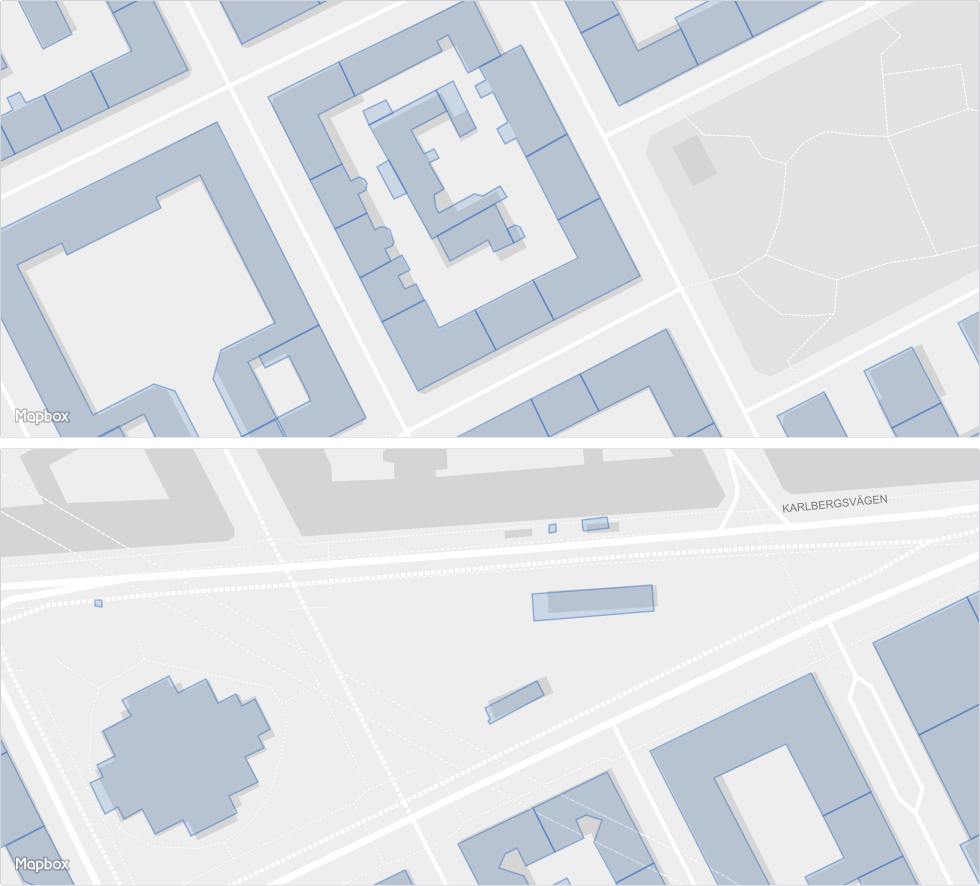
\includegraphics[width=\textwidth,height=0.5\textheight,keepaspectratio]{img_map_compare}
    \caption{Example segments of the Stockholm metropolitan area with unsystematic errors in precision. The SLU building dataset (blue) in superimposed on the OSM dataset (dark gray). The top picture is centered on a city block which shows a semantic mismatching between the two datasets. The whole block consists of only two buildings in the OSM dataset, but is divided into 15 smaller building lots in the SLU dataset. The bottom picture shows 4 smaller buildings whose the positional accuracy is low, due to the buildings being incorrectly scaled, skewed and rotated.}
    \label{fig:space}
\end{figure}

\subsection{The accuracy classes that will not be focused on}

The lineage aspect of the OSM data is available through the OSM History Viewer, an online debugging tool that lets anyone freely view the change history of individual fetures in a commit history-like fashion. There is an option for editors to include a personal note with their changesets to include additional details or motivate why a change was made, but there is no guaratee that the data includes any information on the aquisition method used (OSM 2020). The history aspect of the SLU dataset is not freely available online, but the acquistion method is included in the file metadata on a per-object basis. Lantmäteriet uses internal codes to specifify the acquistion method, and these codes can be referred to in the product description the accompanies the map files. As the scope of this project is limited to making a broad comparison of the positional accuracy of the two datasets, only the required positional accuracy as described by the SLU product description will be used.

The attribute accuracy measure is interesting, as both maps use encoded metadata on a per feature basis, the attribute accuracy of the two datasets could be assessed by doing a simple feature comparison and creating a translation table between the two attribute maps. To the knowledge of the author, this has never been done with specifically these two datasets, at the time of writing.

The temporal accuracy will not be assessed as this projects focuses on comparing a single snapshot of the two datasets at the same point in time.

The logical accuracy will not be assessed because the underlying logical relations between features in both maps serve no purpose to this project.

\subsection{Assesment of dataset completeness}

(Fan et al., 2014) used the total building area in their reference dataset and the OSM dataset to assess the completeness of OSM data. The motivation for this is to eliminate semantic differences between both datasets. A very common example of a semantic error when comparing geographic data is that a large building in one dataset may be segmented into several smaller ones in the other, that is to say a building in one set is represented as an aggreation of mutliple buildings in the other set. This makes one-to-one object mapping impossible. Thus using building area as an estimator for completeness solves this issue much better than i.e. the number of buildings or other objects in each dataset.
This project will use the building area in the OSM dataset versus that of the SLU dataset to determine the completeness of OSM building data in the Stockholm area, which will then be used as an argument for how accurate the building correspondence and point proximity measures can be.

\begin{figure}[H]
    \centering
    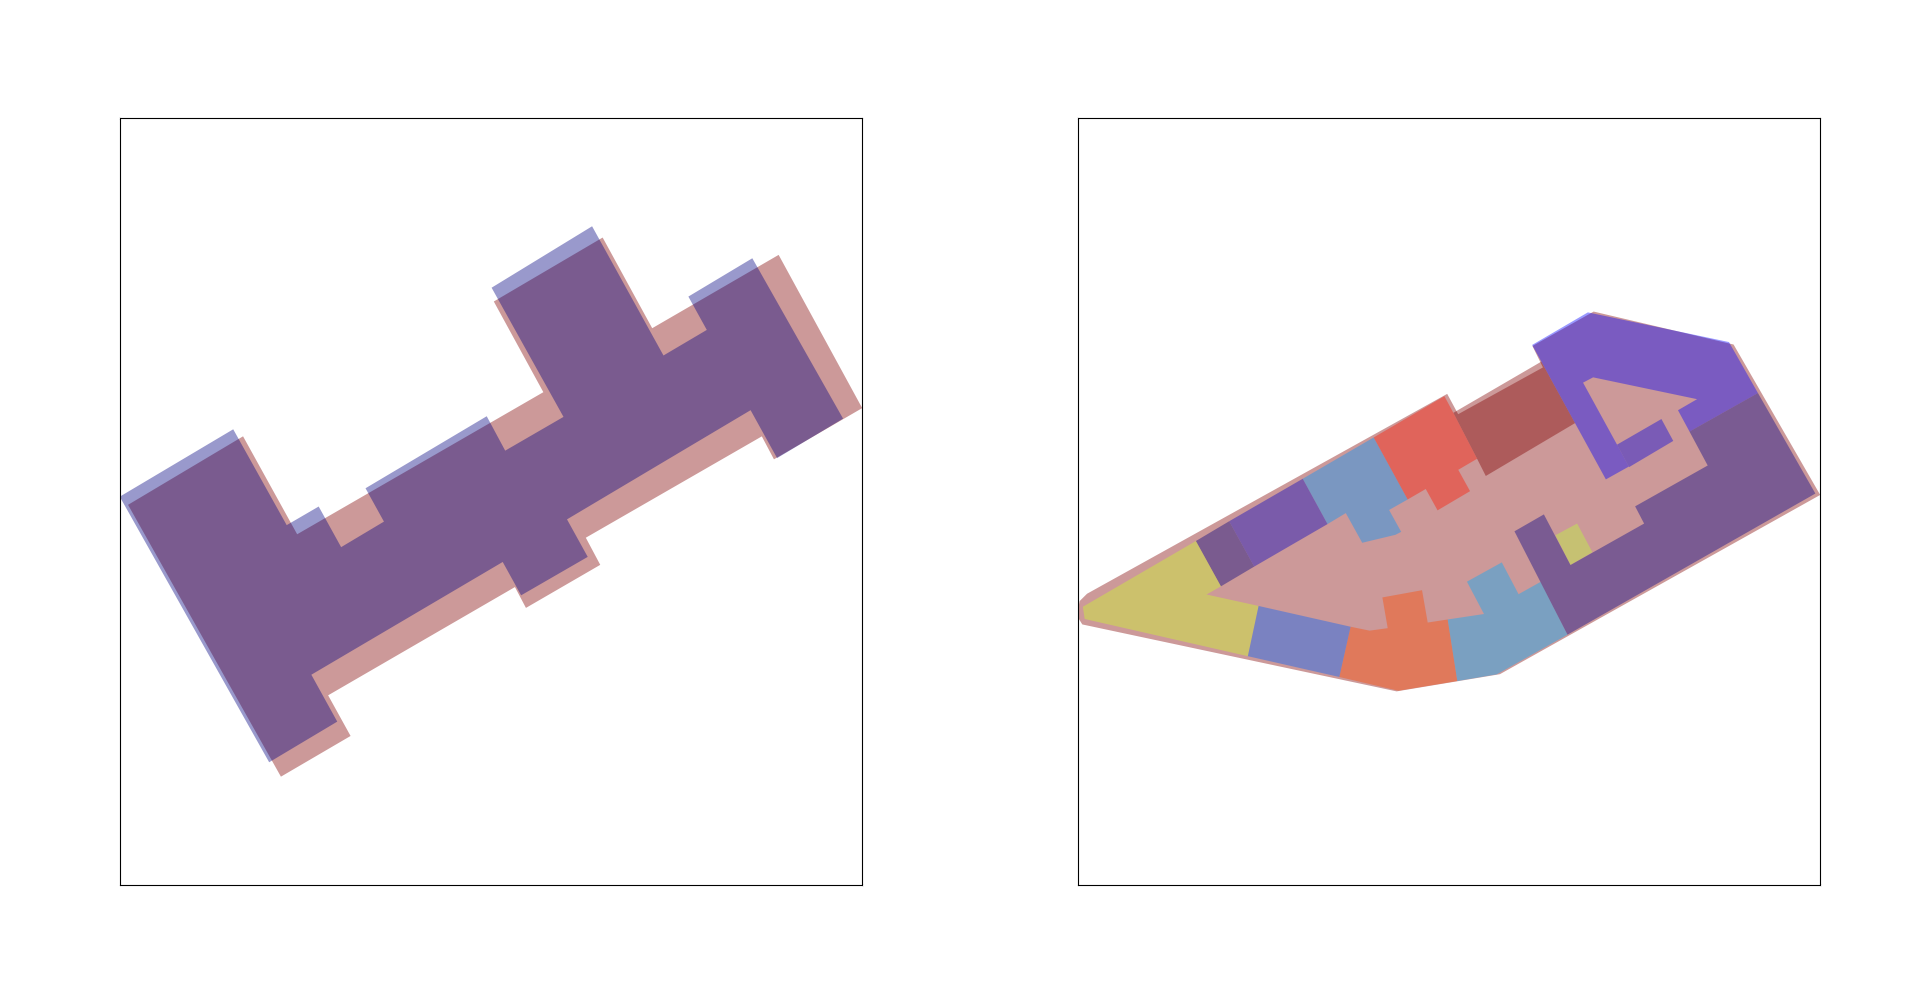
\includegraphics[width=\textwidth,height=0.5\textheight,keepaspectratio]{img_building_match}
    \caption{Examples of a 1:1 building match (left), where the sought-after building was found both in the OSM (red) and SLU (blue) datasets, and of a 1:n building match (right), where the sought-after building was represented as one polygon in the OSM (red) dataset, but divided into many smaller lots in the SLU (multicolored) dataset.}
    \label{fig:space}
\end{figure}

\subsection{Building correspondence}

Feature mapping
The building footprint correspondence will be evaluated using a similarity function that assesses the turning funciton and relative area overlap. The similarity function between any building in the OSM data set and any building in the SLU datasets will be defined as a function of their respective footprints ($foot_{OSM}, foot_{SLU}$), as follows:
\begin{center}
    $S(foot_{OSM}, foot_{SLU}) = S_{T}(foot_{OSM}, foot_{SLU}) + S_{RO}(foot_{OSM}, foot_{SLU})$
\end{center}
where $S_{T}$ measures the difference in turning function and $S_{RO}$ measures the relative overlap between the footprints.

\subsection{Turning function definition}

The turning function was first defined by Arkin et al. (1991), as a method for measuring the similarity of two polygons. The Turning function $T_c(l)$ measures the cumulative angle of the polygon's counter-clockwise tangent, as a function of the cumulative normalized length l. This project uses the turning function as it is defined by (Fan et al., 2014). For a polygon with vertices ${v_1 ... v_n}$ and line segments ${e_1 ... e_n}$ It is defined as follows.
Fix a starting vertex $v_1$.
The tangent angle at $v_1$ is $\theta_{n,1}$. This is the angle between the neighbouring line segments $e_n$ and $e_1$.
For any $i$ such that $i>1$ and $n<i$, the tangent angle at $v_i$ is recursively defined as:
\begin{center}
    $\theta_{i, i-1} = \theta_{n,1} + \sum^{i}_{k=1} \theta_{k, k-1}$
\end{center}
The turning function has some nice geometric properties, in that it is invariant to both rotation and scaling of the polygon. The function contains no information of the orientation of the polygon, only of the relative angle between successive line segments, thus it does not change under roation. It also measures only the normalized cumulative length, which does not change under scaling.
The similarity of two polygons A and B in terms of their turning function is defined as their distance of their cumulative turning functions:
\begin{center}
    $S_{T}(A, B) = 1 - (\int^{1}_{0} T_{C,A}(l) - T_{C,B}(l) dl)^{1/2}$.
\end{center}
The value range will be $(0 < S_{T} < 1)$, where $S_{T}(A,B) = 1$ if the polygons are identical. 

\begin{figure}[H]
    \centering
    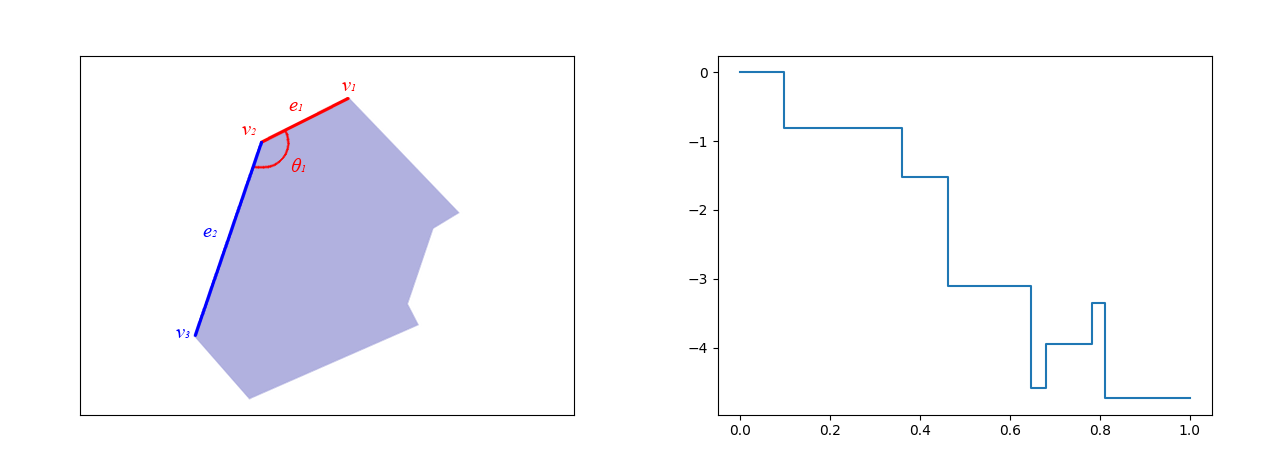
\includegraphics[width=\textwidth,height=0.5\textheight,keepaspectratio]{img_turn_function}
    \caption{An example of the turning function of a polygon.}
    \label{fig:space}
\end{figure}

\begin{figure}[H]
    \centering
    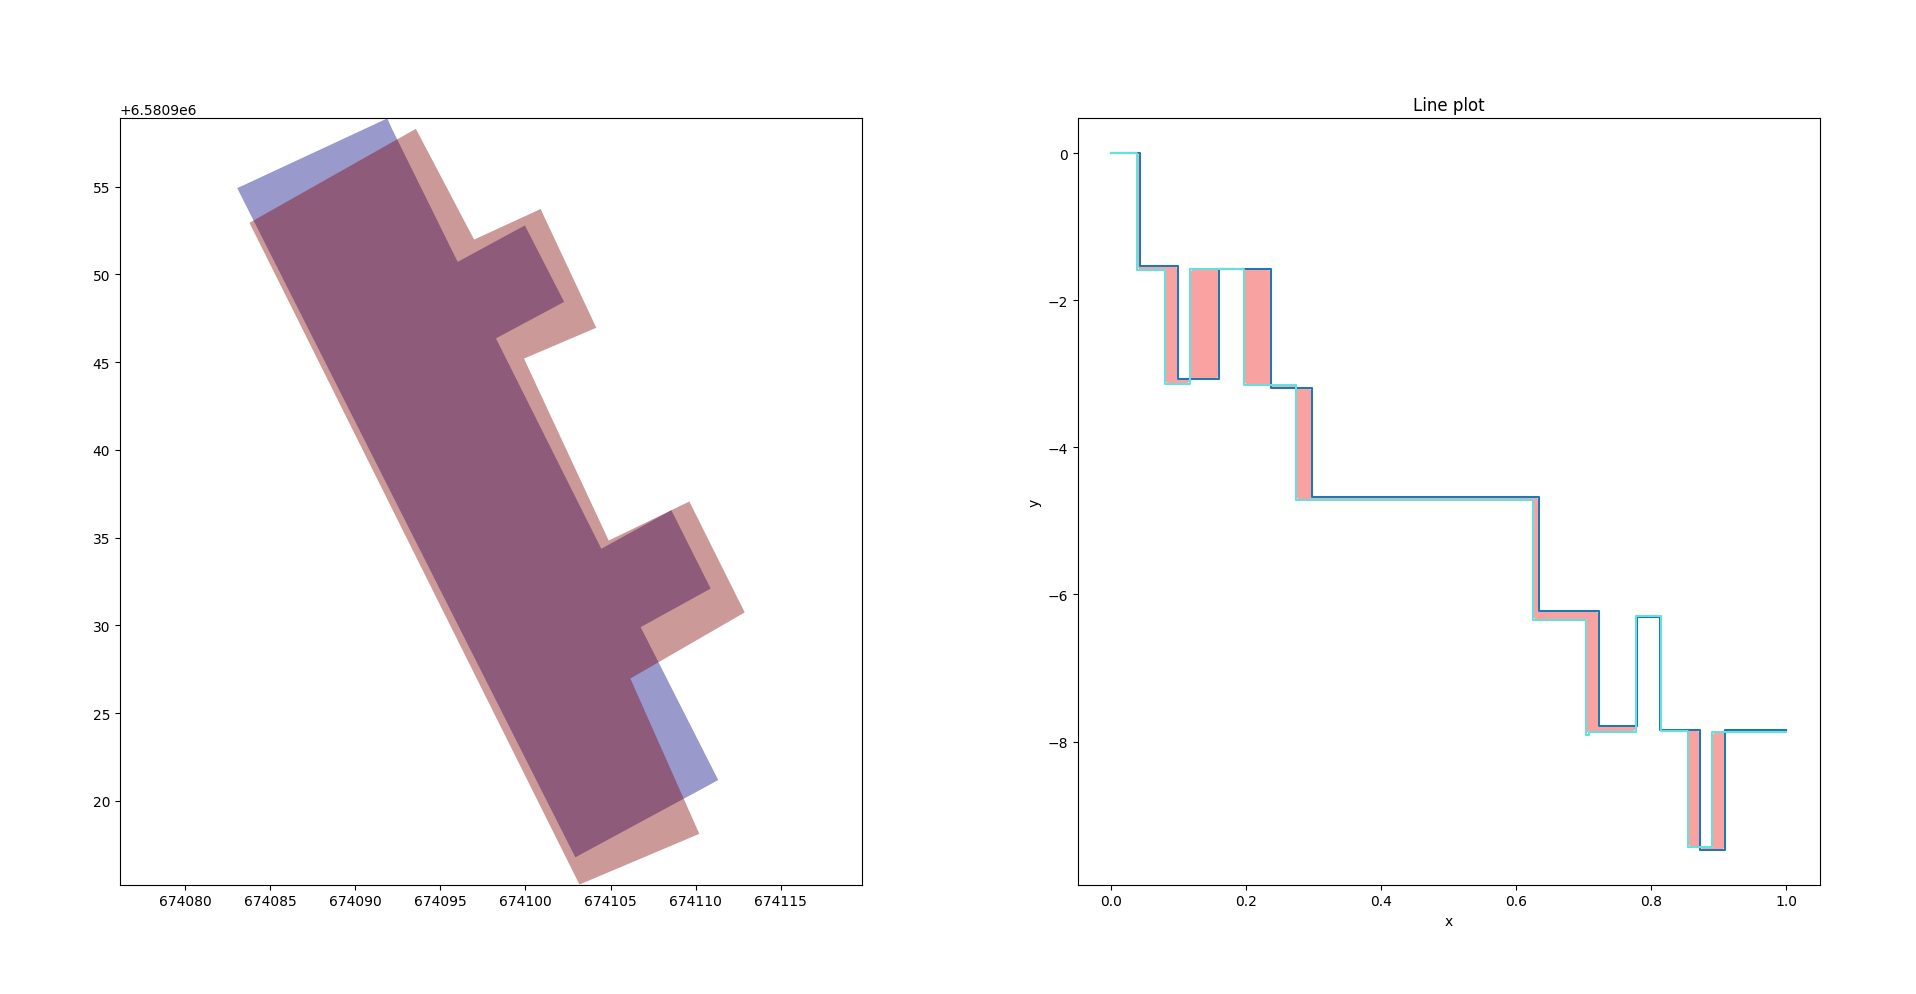
\includegraphics[width=\textwidth,height=0.5\textheight,keepaspectratio]{img_turn_function_diff_filled}
    \caption{An example of the turning functions of two corresponding buildings, with the area between them highlighted.}
    \label{fig:space}
\end{figure}

\subsection{Correspondence by building area}

(Fan et al., 2014) further discussed how the relative overlap in building area can be used to determine building correspondence between datasets, in cases where there is not much displacement between OSM building footprints data and the reference data set. Figure X (TODO) shows a typical comparison between the OSM and SLU datasets, and by eyesight it was determined that the displacement of features is small. The relative building overlap between the OSM and SLU datasets will be defined as folows, given the footprints of any building in the OSM set ($foot_{OSM}$) and the SLU set ($foot_{SLU}$):

\begin{center}
    $S_{RO}(foot_{OSM}, foot_{SLU}) = \frac{A_{Overlap}}{min(A_{foot_{OSM}}, A_{foot_{SLU}}))}$
\end{center}

For this project the relative overlap will be used both to find possible matching building candidates, and as a term in their similarity function.

The relative overlap may be used to determine building matching relations even when the semantic accuracy is low. If a large building is represented by a single footprint in one dataset but by several smaller footprints in the other, (Rutzinger et al, 2009) found that if $S_{RO}(foot_{A}, foot_{B}) < 30\%$ for two buildings $A$ and $B$ from different sets, then $A$ and $B$ are highly likely to be separate, neighbouring buildings and not in fact identical. Therefore we will here assume that two buildings are matching candidates if their relative area overlap is greater than 30\%. If a one-to-many object matching is found, the compound perimeter of the footprints in the many-set will be used when calculating the turning function and finding closest vertices between the polygons.

\subsection{Closest point and point proximity}

The final problem is that even when building polygons have been matched between the two datasets, they may not have one-to-one vertex relationship. Footprints from different datasets may be formed at a different level of detail. Problems that arise are e.g. that the vertex counts are dissimilar, or that vertex clusters may be found at different parts of the polygon in the two datasets. To avoid this effect, key points are extracted using the Douglas-Peucker algorithm (Douglas and Peucker, 1973), to create a simplifed footprint with less points that still retain information about the rough features of the detailed footprint. The idea behind Douglas-Peucker is to recursively divide a polyline. It initially marks only the start and end points $(v_0, v_n)$ to be kept, and finds the point $v_i$ in between whose distance is the greatest to the line segment between $v_0$ and $v_n$. It then recursively refines the line segments $(v_0, v_i)$ and $(v_i, v_n)$, and proceeds to do so until a line segment $(v_j, v_k)$ is found, where every point in between $v_j$ and $v_k$ have a distance to the line segment $(v_j, v_k)$ that is smaller than some resolution $\epsilon$. Then $v_j$ are added to the simplified polyline, and all nodes in between them are discarded. See Algorithm 1 for a detailed view. In either case The Oriented Minimum Bounding Rectangle (MBR) is calculated for the two polygons. Finally the MBR for the OSM building footprint is shifted so that its centroid aligns with the centroid of the MBR of the SLU building footprint. Any edges in the simplified footprints that coinside with the MBR from the same dataset are extracted, and the corresponding points in the original footprints will be matched with each other.

\begin{algorithm}[H]
\SetAlgoLined
\KwResult{Write here the result }
    // Find the point with the maximum distance\;
    $d_{max}$ = 0\;
    $index$ = 0\;
    $end$ = length(PointList)\;
    
    \For{$i$=2 to ($end$-1)}{
        $d$ = perpendicularDistance(PointList[$i$], Line(PointList[1], PointList[$end$]))\;
        \If{$d$ $>$ $d_{max}$} {
            $index$ = $i$\;
            $d_{max}$ = $d$\;
        }
    }

    ResultList = []\;
    
    // If max distance is greater than epsilon, recursively simplify\;
    \eIf{$d_{max}$ $>$ $\epsilon$} {
        // Recursive call\;
        recResults1[] = Douglas-Peucker(PointList[1...$index$], $\epsilon$)\;
        recResults2[] = Douglas-Peucker(PointList[$index$...$end$], $\epsilon$)\;

        // Build the result list\;
        ResultList[] = {recResults1[1...length(recResults1) - 1], recResults2[1...length(recResults2)]}\;
    }{
        ResultList[] = {PointList[1], PointList[$end$]}\;
    }
    \Return{ResultList[]}\;

    \caption{Douglas-Peucker}
\end{algorithm}

Finally, when two building footprints and their vertices have been mapped, we will use the offset of matching vertices as a measure of positional error. The average and variance in vertex spread will be calculated and used to make an assessment of the geometric precision of the OSM dataset, and this precision will further be used to form an upper boundary on geometrical corrections that can be made to the map once it has been imported into the application.

\subsection{Notes about data processing}

Once data from the both sets had been extracted, they looked dissimilar. (Show picture) Had to go over all OSM buildings that intersected with the query box and remove them, along with any SLU buildings that intersected with them.

When calculating the area overlap we used the fact that multipolygons in geojson are represented with the main, bounding polygon first. When calculating the area of a multipolygon building, we simply took the area of the first polygon and subtracted the subsequent ones.

However, when calculating the relative area overlap, this becomes unesseccary since any semantically incorrect subdivision of the polygon will always be inside the bounding polygon.

\section{Collision checks}

% TODO: Write disposition for implementation of the collision checker
The maximum distance between two features was set to 2 times the positional accuracy, since then there will always be ample room to make changes to any features that would collide with the newly noved nodes, and thus we do not need to worry about feature collisions propagating.

In this implementation, roads of different types were allowed to merge into one another to form common intersections. To facilitate this, it was neccessary to work with a path-by-path representation of the point data. When two path share a node with common coordinates, they form an intersection which can be of multiple different types.

The default minimum widths were obtained from (Lantmäteriet, 20). The standard minimum width for a two-lane road in Sweden is 6.5 meters.

Subsequent visual measurements of a few key locations in the Stockholm area revealed the following minimum way widths:
\begin{table}[H]
\begin{tabular}{lllll}
                  & Footpath & Residential & Secondary & Primary \\
    Minimum width & 2.0 m    & 6.0 m       & 6.5 m     & 8.0 m   \\
    Maximum width & 5.0 m    & 9.0 m       & 10.0 m    & 16.0 m
\end{tabular}
\end{table}

\section{Results, Metrics}

\subsection{Completeness by building area}

\begin{table}[H]
\begin{tabular}{lllll}
    & Total number of buildings & Area cover \\
    OSM & 102755 & 33105023.32... $m^2$ \\
    SLU & 170783 & 33718628.97... $m^2$
\end{tabular}
\end{table}

\begin{table}[H]
\begin{tabular}{lllll}
    & Number of buildings (\%) & Area cover (\%) \\
    OSM & 60.17\% & 98.18\% \\
    SLU & 100.00\% & 100.00\%
\end{tabular}
\end{table}

The area cover of the OSM dataset in relation to the SLU dataset was estimated to 98.18\%.

\subsection{Positional accuracy statistics}

\begin{table}[H]
\begin{tabular}{lllll}
    $e_{average}$ & $e_{max}$ & $e_{min}$ & $e_{standard deviation}$ \\
    2.0579... & 9.9878... & 0.0 & 1.2464...
\end{tabular}
\end{table}

Building matching statistics:

\begin{table}[H]
\begin{tabular}{lllll}
    & 1:0 & 1:1 & 1:n & Total \\
    Match count & 9812   & 81722   & 11221   & 102755 \\
    Percent     & 9.55\% & 79.53\% & 10.92\% & 100\%
\end{tabular}
\end{table}

% Bar plot positional accuracy

\begin{figure}[H]
    \centering
    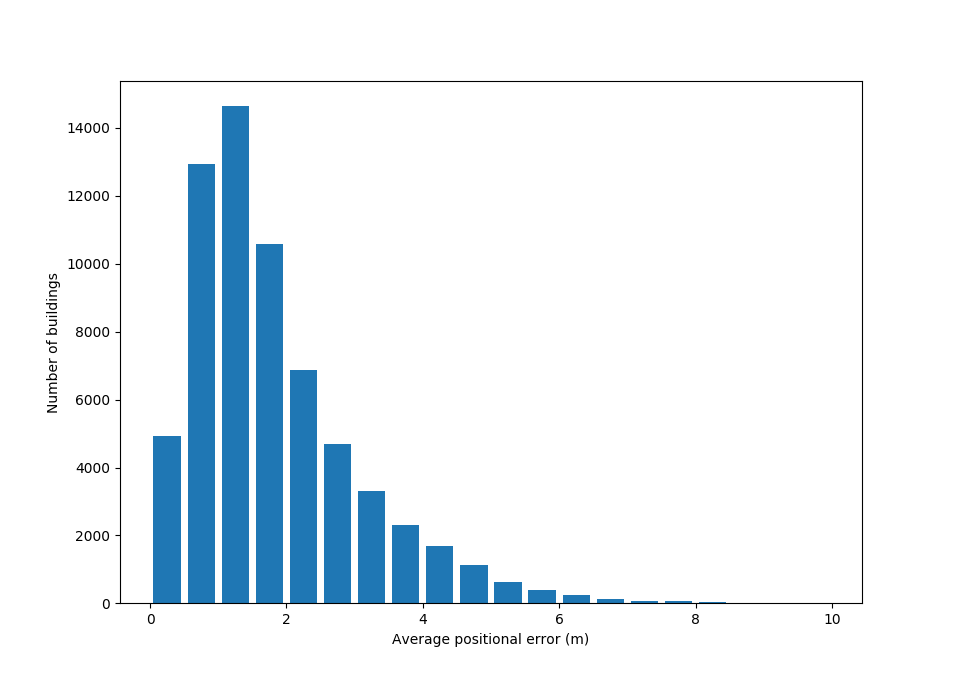
\includegraphics[width=\textwidth,height=0.5\textheight,keepaspectratio]{img_pos_error_plot}
    \caption{The average positional accuracies per building as a frequency diagram.}
    \label{fig:space}
\end{figure}

\subsection{Shape accuracy statistics}

% Bar plot turning functions

\begin{figure}[H]
    \centering
    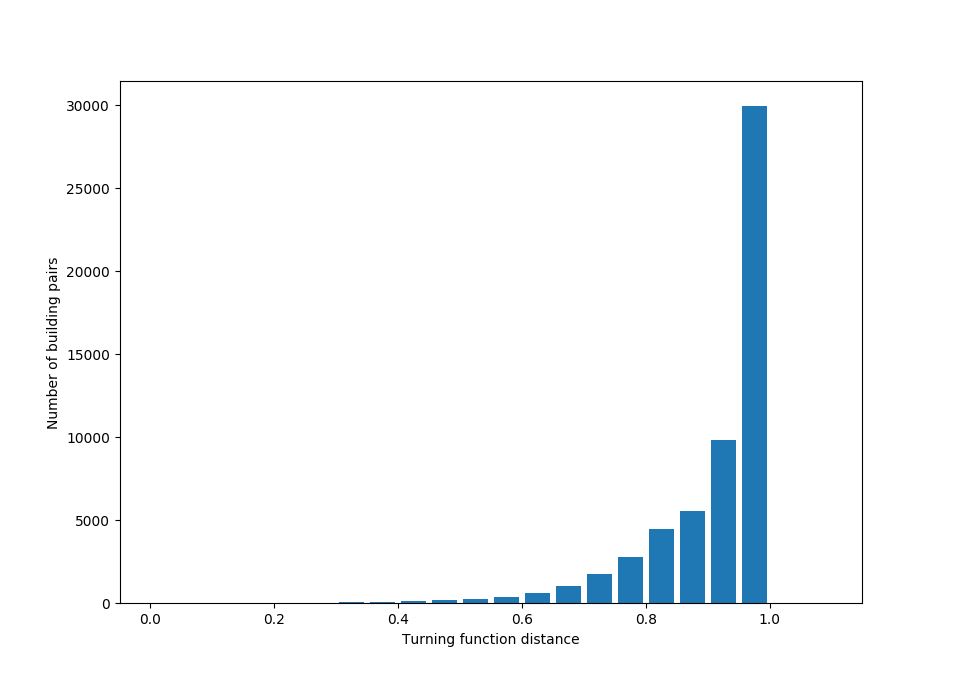
\includegraphics[width=\textwidth,height=0.5\textheight,keepaspectratio]{img_turning_function_plot}
    \caption{The turning function distances between 1:1 building pairs as a frequency diagram.}
    \label{fig:space}
\end{figure}


\subsection{Way collision statistics}

\begin{table}[H]
\begin{tabular}{lllll}
                            & Footpath      & Residential  & Secondary   & Primary     \\
    Features, total         & 26473         & 10523        & 3044        & 2756        \\
    Nodes, total            & 6382579       & 6612383      & 968420      & 420810      \\
    Edge length, total      & 129984.79 km  & 186089.55 km & 29304.57 km & 16162.95 km \\
    Features, colliding     & 3189          & 1032         & 412         & 456         \\
    Nodes, colliding        & 7330          & 2362         & 643         & 824         \\
    Edge length, colliding  & 110.67 km     & 66.18 km     & 9389.30 m   & 20.41 km    \\
    Features, percent       & 12.05 \%      & 9.81 \%      & 13.53 \%    & 16.55 \%    \\
    Nodes, percent          & 0.11 \%       & 0.04 \%      & 0.07 \%     & 0.20 \%     \\
    Edge length, percent    & 0.09 \%       & 0.04 \%      & 0.03 \%     & 0.13 \%

\end{tabular}
\end{table}

After collision correction:

\begin{table}[H]
\begin{tabular}{lllll}
                            & Footpath      & Residential  & Secondary   & Primary     \\
    Features, colliding     & 134           & 336          & 246         & 277         \\
    Nodes, colliding        & 157           & 530          & 306         & 407         \\
    Edge length, colliding  & 3248.73       & 6475.99 m    & 3840.00 m   & 8039.54 m   \\
    Features, percent       & 0.51 \%       & 3.19 \%      & 8.08 \%     & 10.51 \%    \\
    Nodes, percent          & 0.00 \%       & 0.00 \%      & 0.03 \%     & 0.09 \%     \\
    Edge length, percent    & 0.00 \%       & 0.00 \%      & 0.01 \%     & 0.05 \%

\end{tabular}
\end{table}

\section{Analysis and Future Work}

\subsection{Quality of the OSM dataset}

Accuracy: we can assume that Stockholm, being one of the more developed cities in one of the most technologically connected country in the world, would be fairly well mapped in OSM. The positional accuracy has improved by roughly 3.5 meters since the study by (Haklay, 2010), and by roughly 1.5 meters since the study by (Fan et al, 2014), if the SLU reference dataset is to be believed as absolute.

The completeness analysis by building area shows that the OSM Stockholm dataset has high completeness in terms of both building area and counted features, in the same level as the study of Munich by (Fan et al, 2014).

The difference in area cover can partially be explained by small utility buildings that are often not represented in the OSM dataset. Particularily the residential areas in downtown, Stockholm, are characteristic in that each city block consists of a street front and an open, communal compound in the middle, inside of which there are usually a number of small utility buildings such as bicycle garages, toolsheds, refuse rooms and such. These buildings are likely hard to make out and trace on publicly available satellite image data. They are, according to (Fan et al, 2014) occluded by their surroundings due to shadows or forestry. This appears to be a large consensus in the field.

The low semantic accuracy has made analysis hard. The available SLU dataset from Lantmäteriet uses a plot-based subdivision of buildings, whereas OSM uses a subdivision that more closely resembles the actual building footprint as seen from above. In many cases whole city blocks are represented as single buildings, which means that many less meaningful feature matches can be found.
As seen in table ***, about 80\% of all OSM features were found to have a 1:1 mapping to the SLU dataset, but upon further visual comparison it can be seen that many of the 1:n matches are found in a very specified area, namely the residential areas in downtown, Stockholm. This is problematic since this typical area with the same level of accessibility was likely measured with the same measuring technique, and the unsystematic positional error will likely be similar in these areas. The question is wether it comforms well to the positional error in the rest of the dataset or not. This analysis will not be carried out in this project, but could be a good subject for a future master's thesis project.

\begin{figure}[H]
    \centering
    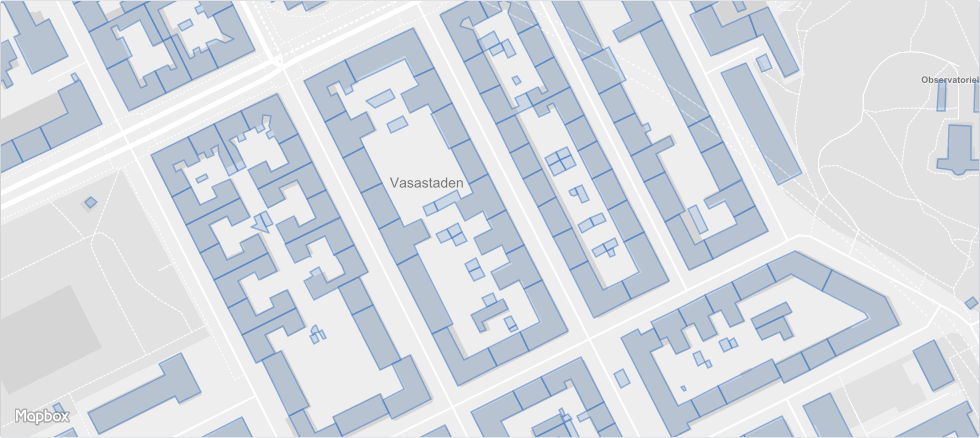
\includegraphics[width=\textwidth,height=0.5\textheight,keepaspectratio]{img_map_utility_buildings}
    \caption{A map segment which shows an area with many small utility buildings that are represented in the SLU dataset but not in the OSM dataset.}
    \label{fig:space}
\end{figure}

\subsection{Utility in real world applications}

% TODO: Interview with Todor

\subsection{Feature overlap}

After visual inspection of the cases where features collide, it was determined that all collision occurences can be almost exclusively classified into one of five categories:

\begin{enumerate}
\item Case 1: A building lies in paralel with a road, and the distance between the two is smaller than the minimum width of the road.
\item Case 2: A road shares a node with a building.
\item Case 3: A road is intersecting with certain building features.
\item Case 4: Two roads have a minimum distance that is smaller than the sum of the minimum widths of both roads. 
\item Case 5: Two roads share a node, and a subsequent node in one road lies within the minimum width of the other road.
\end{enumerate}

Each case is exemplified in figure X. %{TODO}

\begin{figure}[H]
    \centering
    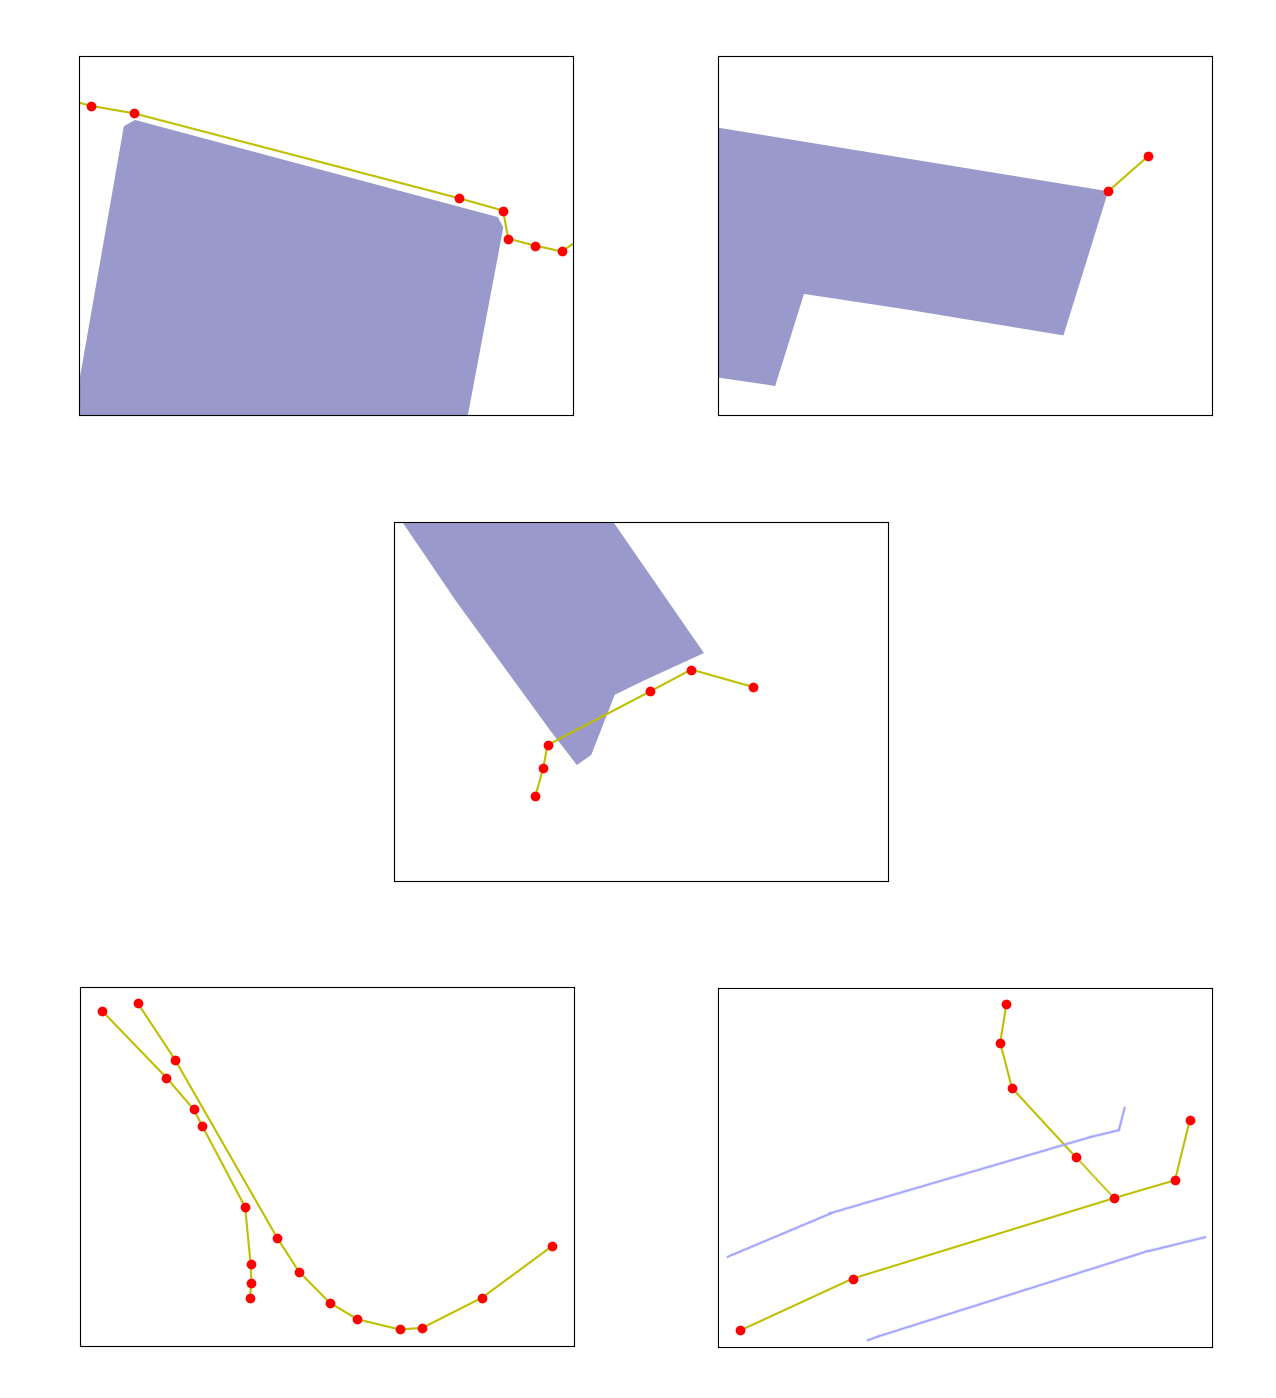
\includegraphics[width=\textwidth,height=0.5\textheight,keepaspectratio]{img_feature_overlap_cases}
    \caption{The 5 identified cases over feature overlap. Top left: Case 1. Top right: Case 2. Middle: Case 3. Bottom left: Case 4. Bottom right: Case 5.}
    \label{fig:space}
\end{figure}

All these cases will create issues when generating the 3D mesh representation of the city.
Conslusion: footpaths were not worse than other categories, which are included in many unity packages already

Propagation of error, have to include all the edited features in the next pass

(Fan et al, 2014) claimed that the positional error is largely due to the limited resolution in satellite imagery.

\subsection{Suggested algorithms for correcting feature overlap}

All collision cases can be solved with relatively simply geometric algorithms. This section will present suggestions on algorithms that will resolve collisions by identifying individualcolliding nodes and translating them, after which some degree of smoothing (such as linear interpolation) can be applied to preserve visual features. Cases 1 and 3-5 will be handled, while 2 will be left since case 2 collisions do not inherently cause feature overlap when extruding a 3D road mesh from the way edges. Thus it will me up to the individual developer to decide what to do with Case 2 collisions.

\begin{figure}[H]
    \centering
    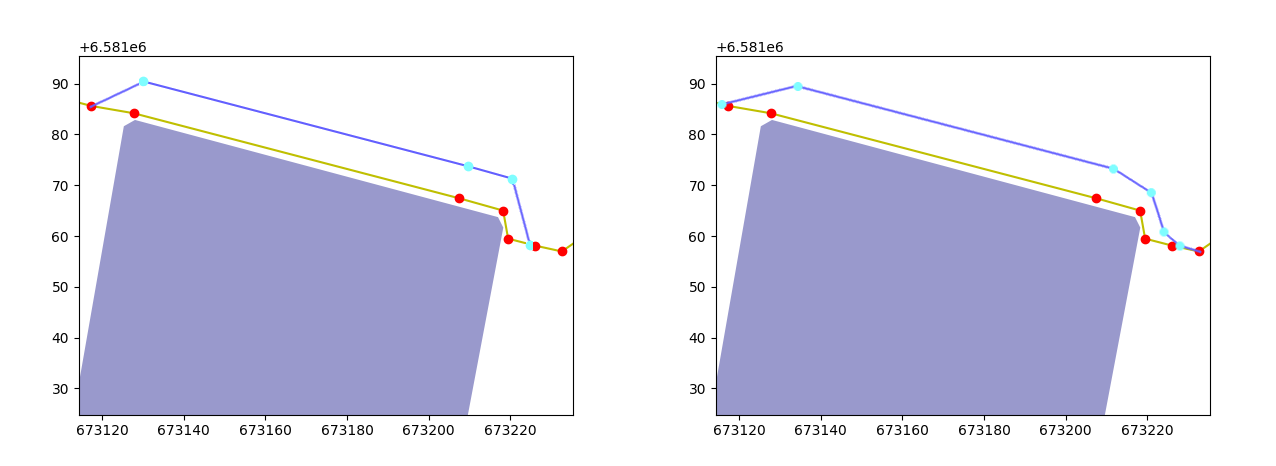
\includegraphics[width=\textwidth,height=0.5\textheight,keepaspectratio]{img_feature_overlap_fix_1}
    \caption{Case 1 collisions can be solved by translating colliding way points away from the building, along the normal of the nearest surface. Smoothing can then be applied as seen fit.}
    \label{fig:space}
\end{figure}

\begin{figure}[H]
    \centering
    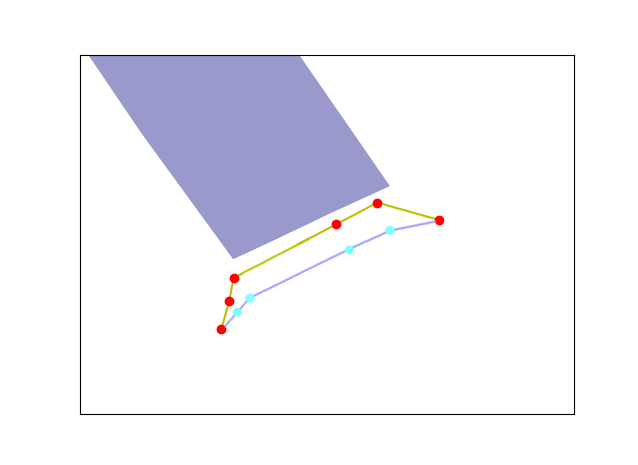
\includegraphics[width=\textwidth,height=0.5\textheight,keepaspectratio]{img_feature_overlap_fix_2}
    \caption{Case 3 collisions can be solved by eliminating the building features that intersect with the way, and then applying the same algorithm as in case 1.}
    \label{fig:space}
\end{figure}

\begin{figure}[H]
    \centering
    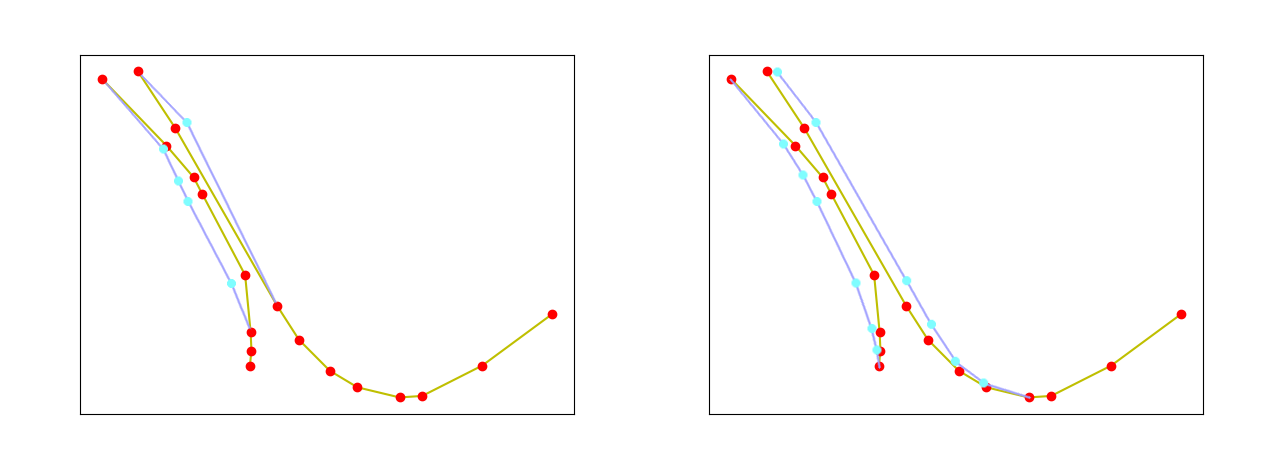
\includegraphics[width=\textwidth,height=0.5\textheight,keepaspectratio]{img_feature_overlap_fix_3}
    \caption{Case 4 collisions can be solved by calculating the average normal over all colliding edges for both ways, and translating colliding points along the normal, away from the other way. Smoothing can then be applied as seen fit.}
    \label{fig:space}
\end{figure}

\begin{figure}[H]
    \centering
    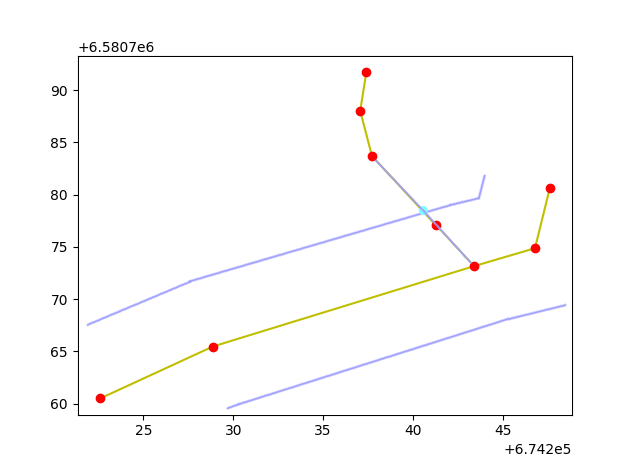
\includegraphics[width=\textwidth,height=0.5\textheight,keepaspectratio]{img_feature_overlap_fix_4}
    \caption{Case 5 collisions can be solved simply by translating the colliding point along the tangent of the closest edge, and then applying smoothing as seen fit.}
    \label{fig:space}
\end{figure}


\begin{thebibliography}{9}

\bibitem{lantmateriet-19}
(Lantmäteriet, 2019), Produktbeskrivning: GSD-Fastighetskartan vektor \\ 
\href{https://www.lantmateriet.se/globalassets/kartor-och-geografisk-information/kartor/fastshmi.pdf}.

\bibitem{osm-19}
(OSM 19) Converting to WGS84, accessed 13-03-2020 \\ 
\href{https://wiki.openstreetmap.org/wiki/Converting\_to\_WGS84}.

\bibitem{osm-20}
(OSM 20) OSM History Viewer\\
\href{https://wiki.openstreetmap.org/wiki/OSM\_History\_Viewer}.

\bibitem{haklay-10}
(Haklay, 2010), How good is volunteered geographical information?A comparative study of OpenStreetMap and OrdnanceSurvey datasets \\
\href{https://kfrichter.org/crowdsourcing-material/day1/haklay10.pdf}.

\bibitem{fan-14}
(Fan et al, 2014), Quality assessment for building footprints data on OpenStreetMap \\
\href{https://www.researchgate.net/publication/262163378\_Quality\_assessment\_for\_building\_footprints\_data\_on\_OpenStreetMap}.

\bibitem{arkin-91}
Arkin E.M., Chew L.P., Huttenlocher D.P., Kedem K. and Mitchell J.S.B. 1991. An Efficiently Computable \\
Metric for Comparing Polygonal Shapes. In: IEEE Transaction on Pattern Analysis and Machine \\
Intelligence, Vol. 13, No. 3, March 1991. \\

\bibitem{douglas-peucker-73}
Douglas, D.H. and Peucker T.K. 1973. Algorithms for the reduction of the number of points required to \\
represent a digitalized line or its caricature. In: Cartographica: The International Journal for Geographic \\
Information and Geovisualization, 10(2), 112-122. \\

\bibitem{rutzinger-09}
Rutzinger, M., Rottensteiner, F. and Pfeifer, N. 2009. A Comparison of Evaluation Techniques for Building \\
Extraction From Airborne Laser Scanning. IEEE Journal of Selected Topics in Applied Earth \\
Observations and Remote Sensing 2(1): 11-20. \\

\bibitem{trafikverket-20}
https://trafikverket.ineko.se/Files/sv-SE/71830/Ineko.Product.RelatedFiles/2020\_029\_vagar\_och\_gators\_utformning\_krav.pdf \\

\bibitem{stojanovski-20}
Stojanivski T. 2020. Viewpoint: City Information Modeling (CIM) And Digitizing Urban Design Practises.
Under review

\bibitem{van-oort-06}
van Oort P A J. 2006. Spatial Data Quality: From Description to Application. PhD Thesis, Wageningen University.

\bibitem{kunze-12}
Kunze, C. 2012. Vergleichsanalyse des Gebäudedatenbestandes aus OpenStreetMap mit amtlichen Datenquellen. \\
Student research project at the Technical University of Dresden, online avaiable: http://nbn- \\
resolving.de/urn:nbn:de:bsz:14-qucosa-88141

\end{thebibliography}


\end{document}
